\documentclass[10pt]{beamer}
\usetheme[
%%% options passed to the outer theme
%    progressstyle=fixedCircCnt,   %either fixedCircCnt, movCircCnt, or corner
%    rotationcw,          % change the rotation direction from counter-clockwise to clockwise
%    shownavsym          % show the navigation symbols
  ]{AAUsimple}

\usepackage{caption}
\captionsetup[figure]{labelformat=empty}%
\usepackage{graphicx}
  
% If you want to change the colors of the various elements in the theme, edit and uncomment the following lines
% Change the bar and sidebar colors:
%\setbeamercolor{AAUsimple}{fg=red!20,bg=red}
%\setbeamercolor{sidebar}{bg=red!20}
% Change the color of the structural elements:
%\setbeamercolor{structure}{fg=red}
% Change the frame title text color:
\setbeamercolor{frametitle}{fg=white}
% Change the normal text color background:
%\setbeamercolor{normal text}{fg=black,bg=gray!10}
% ... and you can of course change a lot more - see the beamer user manual.

\usepackage[utf8]{inputenc}
\usepackage[english]{babel}
\usepackage[T1]{fontenc}
% Or whatever. Note that the encoding and the font should match. If T1
% does not look nice, try deleting the line with the fontenc.
\usepackage{helvet}

% colored hyperlinks
\newcommand{\chref}[2]{%
  \href{#1}{{\usebeamercolor[bg]{AAUsimple}#2}}%
}

\title{Listen to your Heart:}

\subtitle{Heartbeat Sound Segmentation \& Classification}  % could also be a conference name

\date{\today}

\author{
  Boikanyo Radiokana \& Elias Sepuru  
 % \href{mailto:jkn@es.aau.dk}{{\tt jkn@es.aau.dk}}
}

% - Give the names in the same order as they appear in the paper.
% - Use the \inst{?} command only if the authors have different
%   affiliation. See the beamer manual for an example

\institute[
  {
\includegraphics[scale=0.2]{AAUgraphics/eie.png}}\\ %insert a company, department or university logo
 School of Electrical \& Information Engineering\\ University of the Witwatersrand \\
 South Africa
] % optional - is placed in the bottom of the sidebar on every slide
{% is placed on the bottom of the title page
  School of Electrical \& Information Engineering\\ University of the Witwatersrand \\
  South Africa
  
  %there must be an empty line above this line - otherwise some unwanted space is added between the university and the country (I do not know why;( )
}

% specify a logo on the titlepage (you can specify additional logos an include them in 
% institute command below
\pgfdeclareimage[height=2.0cm]{titlepagelogo}{AAUgraphics/EIElogo.png} % placed on the title page
%\pgfdeclareimage[height=1.5cm]{titlepagelogo2}{AAUgraphics/aau_logo_new} % placed on the title page
\titlegraphic{% is placed on the bottom of the title page
  \pgfuseimage{titlepagelogo}
%  \hspace{1cm}\pgfuseimage{titlepagelogo2}
}

\begin{document}
% the titlepage
{\aauwavesbg%
\begin{frame}[plain,noframenumbering] % the plain option removes the header from the title page
  \titlepage
\end{frame}}
%%%%%%%%%%%%%%%%

% TOC
\begin{frame}{Agenda}{}
\tableofcontents
\end{frame}
%%%%%%%%%%%%%%%%

\section{Introduction}
% Ditumedišo le Matseno
\begin{frame}{Introduction}{}
\begin{block}{}
	
  \begin{columns}
  	\column{0.5\textwidth}
  	\begin{itemize}
  		\item<1-4> CVDs are the leading causes of death globally - WHO.
  		\item<2-4> Currently used method to check for CVDs is Cardiac Auscultation (CA).
  		\item<3-4> CA is a difficult skill to acquire.
  		\item<4-4> People are not aware of their heart conditions.
  	\end{itemize}
  	\column{0.5\textwidth}
  	
  	 \only<1>{ 
  	 	
  	 	\begin{figure}[t]
  	 		
  	 		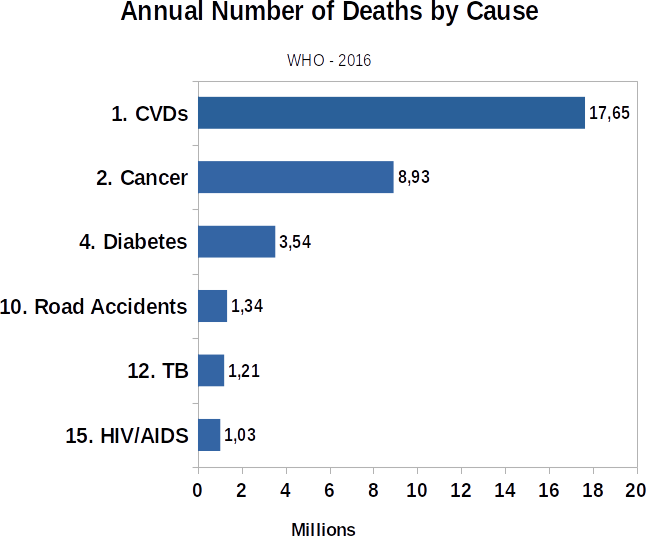
\includegraphics[width=\textwidth,height=0.6\textheight]{AAUgraphics/who.png}
  	 	\end{figure}
  	 }
  	
  	 
  	 % Image on second step
  	 
     \only<2>{ 
     	
     	\begin{figure}
  	 		\centering
  			
\includegraphics[scale=0.20]{AAUgraphics/ausc3.png}
  			
  		\end{figure}
      }
     
      % Image on 3rd step
  
      \only<3>{ 
    	
    	\begin{figure}
    		\centering
    		
\includegraphics[scale=1]{AAUgraphics/confused.jpg}
    	\end{figure}
           
           \vspace{-0.8cm}
           
        \begin{figure}
        	
        	\centering
        	
\includegraphics[width=\textwidth]{AAUgraphics/confstats.png}
        	\caption{\scalebox{.6}{Correct diagnosis using CA  in USA, Canada \& UK respectively.}}
        
        \end{figure}
    	}
    
       % Image on 4th Step
       
       \only<4>{ 
       	
       	\begin{figure}[t]
       		
       		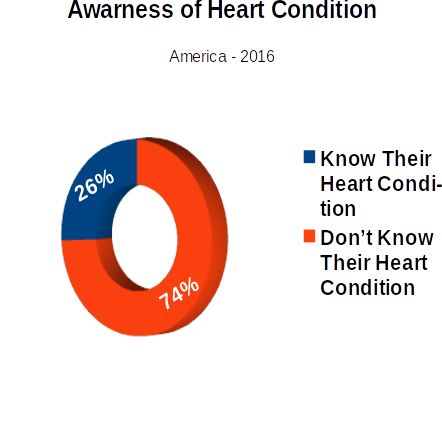
\includegraphics[width=\textwidth,height=0.7\textheight]{AAUgraphics/aware2.png}
       		
       	\end{figure}
       }
   
   
  \end{columns}

  \only<5>{
  	\vspace{-0.8\textheight}
   
     {\Large Easily accessible \& reliable heart diagnosis systems would help reduce deaths due to CVDs.}

     }
  
\end{block}
\end{frame}
%%%%%%%%%%%%%%%%

	%\subsection{License}
	%% the license
	%\begin{frame}{Introduction}{License}
	%  \begin{itemize}
	%
	%  \end{itemize}
	%\end{frame}
	
%%%%%%%%%%%%%%%%

\section{Objectives}
% Kgwekgwe ya taba.
\begin{frame}{Objectives}

	\begin{itemize}
	
		\item<1-> To segment Heartbeat sounds (HSs) based on the location \\of S1 (lub) S2 (dub) in Normal HSs.
	

	\end{itemize}
	{	\begin{figure}
			\centering
			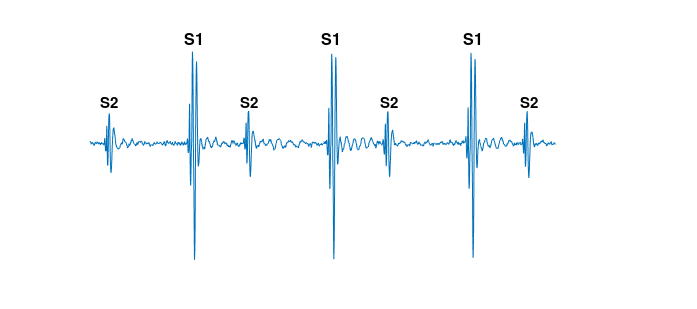
\includegraphics[width=0.75\textwidth,height=0.25\textheight]{AAUgraphics/s1s2s1wc.png}
		\end{figure}
	}

   \pause
   
   \begin{itemize}
   	
   		\item<2-> Create models that will enable preliminary screening of CVDs	
   	
   \end{itemize}
   
   	{	\begin{figure}
   			\centering
   			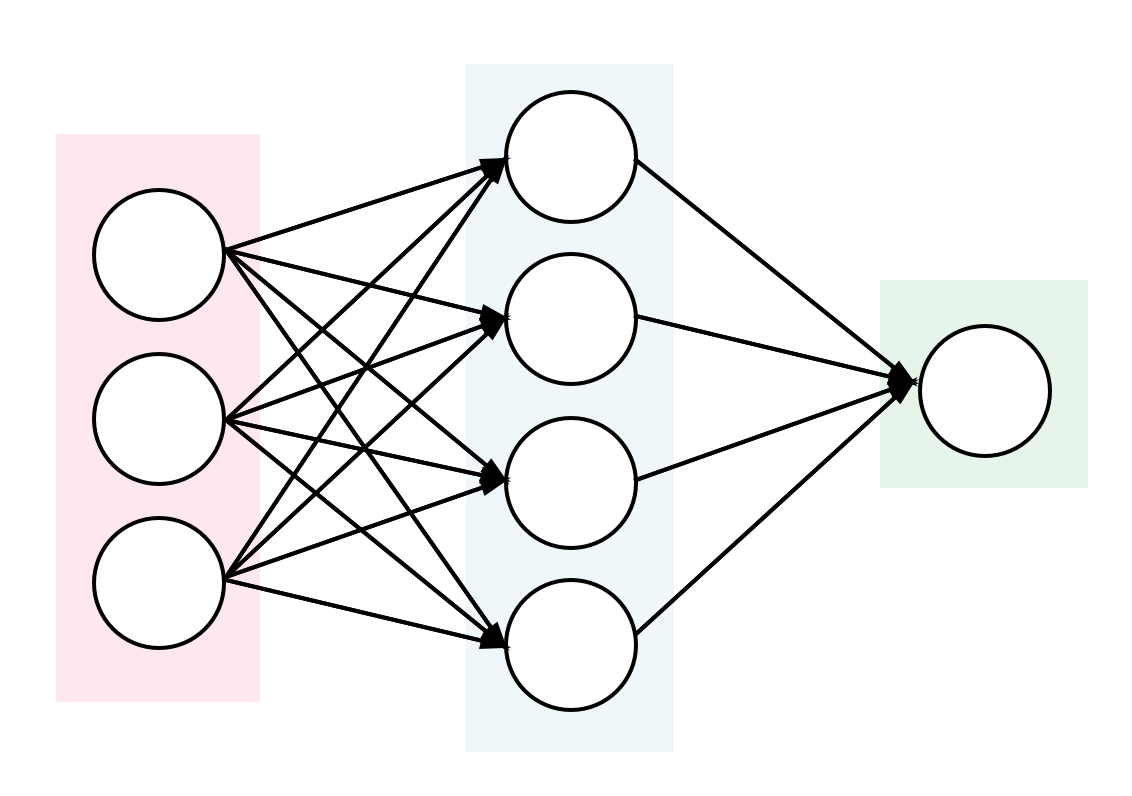
\includegraphics[width=0.5\textwidth,height=0.35\textheight]{AAUgraphics/classification2.png}
   		\end{figure}
   	}


\end{frame}

%%%%%%%%%%%%%%%%

\section{Background}

\subsection{Heartbeat Sounds Categories}
% Mafapha

\begin{frame}{Background}{Heartbeat Sounds Categories}


	
 This project deals with classifying HSs into the following categories:
  
  \begin{enumerate}
  	\item Normal HSs
  	\item Murmur HSs
  	\item Extra Heartsounds
  	\item Exrasystole HSs
  	\item Artifact
  \end{enumerate}


\end{frame}


\begin{frame}{Background}{Heartbeat Sounds Categories}

  \only<1>{ % Tša go loka
	
	\begin{block}{Normal HSs}
		
		\vspace{1cm}
		\hspace{0.25\textwidth}{\texttt{lub...dub......lub...dub.....}}

		\begin{figure}
			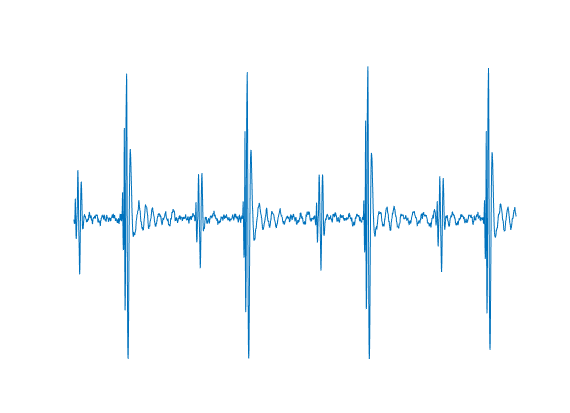
\includegraphics[width=0.8\textwidth,height=0.5\textheight]{AAUgraphics/normal.png}
		\end{figure}

		\end{block}

	}

    \only<2>{ % Bolwetši fela mo!
     	
     	\begin{block}{Murmur HSs}
        \vspace{0.5cm}
     	\hspace{0.18\textwidth}{\texttt{lub..***..dub......lub..***..dub......}}
     	
     	\hspace{0.45\textwidth} or 
     	
     	\hspace{0.18\textwidth}{\texttt{lub....dub...***...lub....dub...***...}}
     	
     		\begin{figure}
     		
     			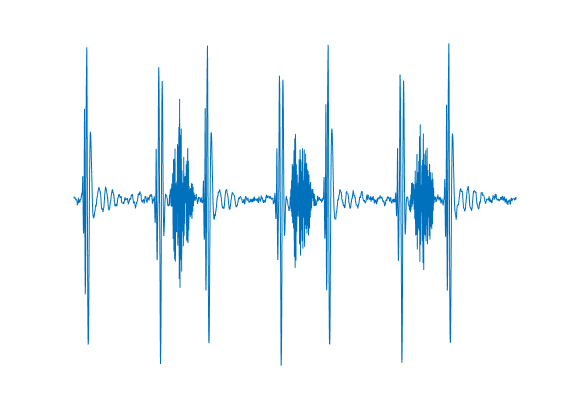
\includegraphics[width=0.8\textwidth,height=0.5\textheight]{AAUgraphics/murmur.png}
     		
     		\end{figure}
     	\end{block}
      
      }
  
  \only<3>{ % O kgaufi le go lwala
  	
  	\begin{block}{Extra HS}
  		
  		\vspace{0.5cm}
  		
  		\hspace{0.2\textwidth}{\texttt{lub.lub...dub.....lub.lub...dub.....}}
  		
  		\hspace{0.45\textwidth} or 
  		
  		\hspace{0.2\textwidth}{\texttt{lub...dub.dub.....lub...dub.dub.....}}
  		
  		\begin{figure}
  			
  			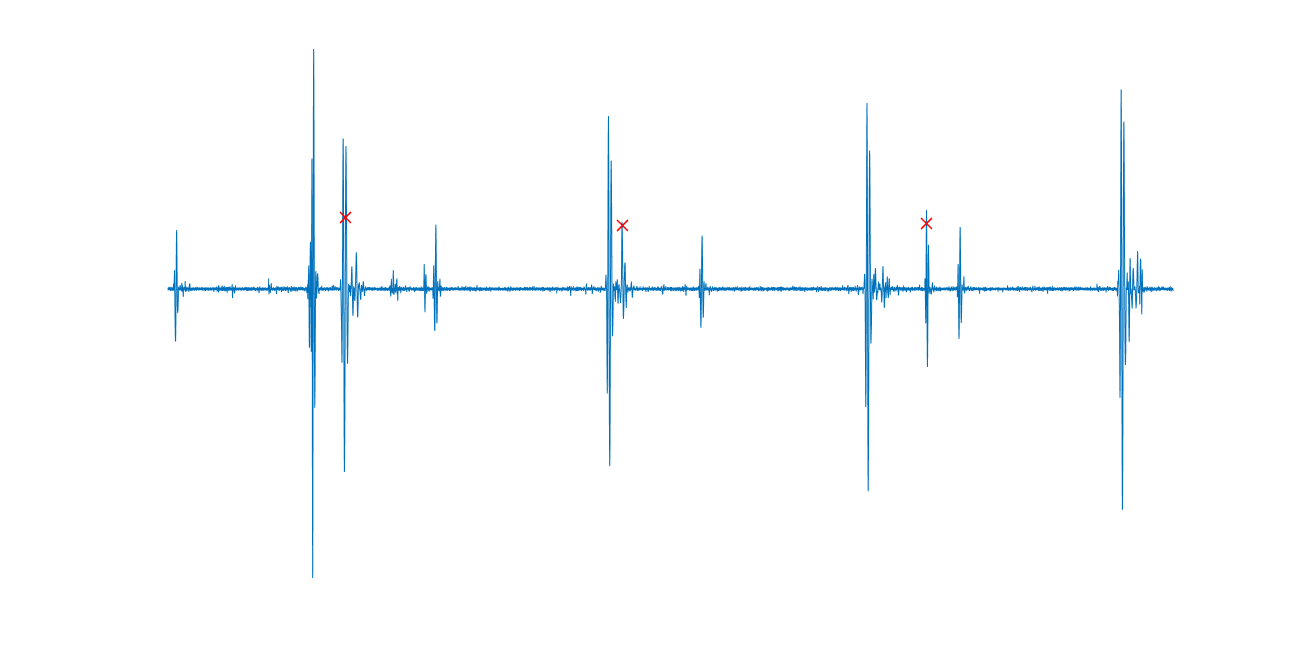
\includegraphics[width=0.8\textwidth,height=0.5\textheight]{AAUgraphics/extra.png}
  			
  		\end{figure}
  	\end{block}
  	
  }

  \only<4>{ % O kgaufi le go lwala
 	
 	\begin{block}{Extrasytole HSs}
 		
 		\vspace{0.5cm}
 		
 		\hspace{0.17\textwidth}{\texttt{lub....dub......lub.lub...dub.....lub....}}
 		
 		\hspace{0.45\textwidth} or 
 		
 		\hspace{0.17\textwidth}{\texttt{lub....dub.dub.....lub...dub......lub....}}
 		
 		\begin{figure}
 			
 			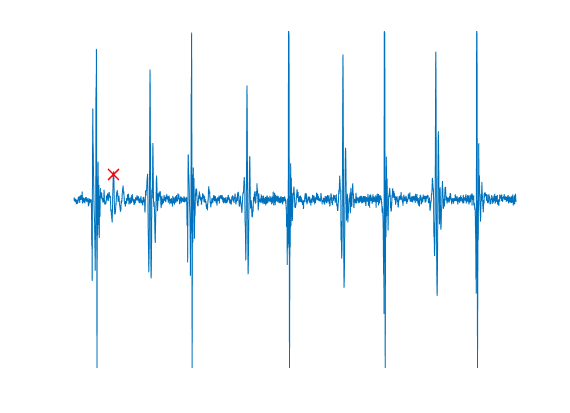
\includegraphics[width=0.8\textwidth,height=0.5\textheight]{AAUgraphics/extrasys.png}
 			
 		\end{figure}
 	\end{block}
 	
 }
 
 
  \only<5>{ % O nyaka go re dira dibari?
 	
 	\begin{block}{Artifact Sound}
 		
 		Not an actual HSs.
 		
 		\begin{figure}
 			
 			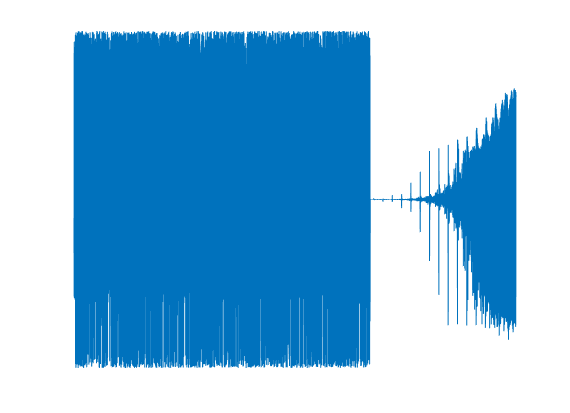
\includegraphics[width=0.8\textwidth,height=0.5\textheight]{AAUgraphics/arti.png}
 			
 		\end{figure}
 	\end{block}
 	
 }
 
\end{frame}


\begin{frame}{Background}{Heartbeat Sounds Categories}

	\begin{block}{Can you guess the categories?}
		
	
         \vspace{-0.25cm}
		\begin{figure}
			A
			
			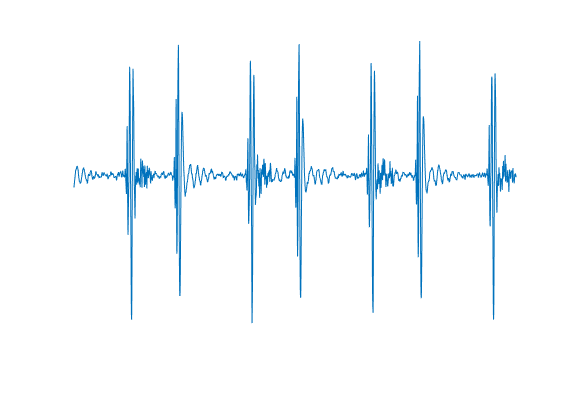
\includegraphics[width=0.8\textwidth,height=0.45\textheight]{AAUgraphics/question.png}
		
		\end{figure}
	
	   \vspace{-2.0cm}
		\begin{figure}
			B
			\vspace{-0.04cm}
		
			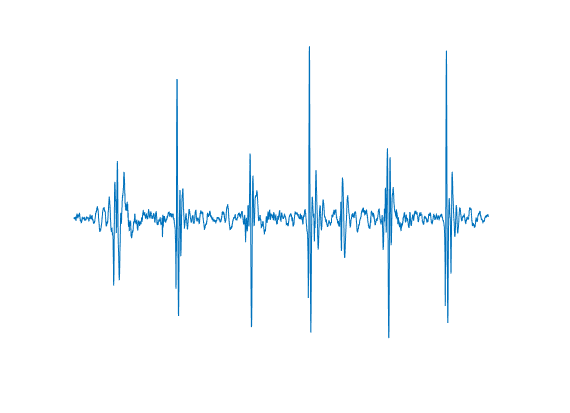
\includegraphics[width=0.8\textwidth,height=0.40\textheight]{AAUgraphics/question2.png}
		
		\end{figure}
	
     \end{block}

\end{frame}

%% 

\subsection{Related Work}

\begin{frame}{Background}{Related Work}

\begin{block}{Strunic's attempt to classify HSs with ANN.}
	
	\begin{columns}
		
		\column{0.5\textwidth}
		    \vspace{0.3cm}
			\begin{figure}
			
\includegraphics[width=0.8\textwidth,height=0.2\textheight]{AAUgraphics/strunic8.png}
				\caption{Accuracy when classifying simulated HSs with no noise.}
		\end{figure}
	
	
	
		\column{0.5\textwidth}
		
			\begin{figure}
			
\includegraphics[width=0.9\textwidth,height=0.25\textheight]{AAUgraphics/strunic42.png}
			\caption{Accuracy when classifying real life HSs with noise.}
		\end{figure}
		

     
    \end{columns}

		
	\end{block}
	
\end{frame}


\subsection{Project Setting}

\begin{frame}{Background}{Project Setting}

\begin{block}{}
	
	
	  {\Large To make this project applicable to real world situations, two datasets recorded in real life settings will be used. Both datasets contain excessive background noise.}
		
\end{block}

\end{frame}


\section{Methodology}

\subsection{Data Acquisition}

\begin{frame}{Methodology}{Data Acquisition}

\only<1>{
	
	\begin{block}{Dataset A}
		
		\begin{columns}
			\column{0.5\textwidth}
			
			\begin{figure}
				\centering
				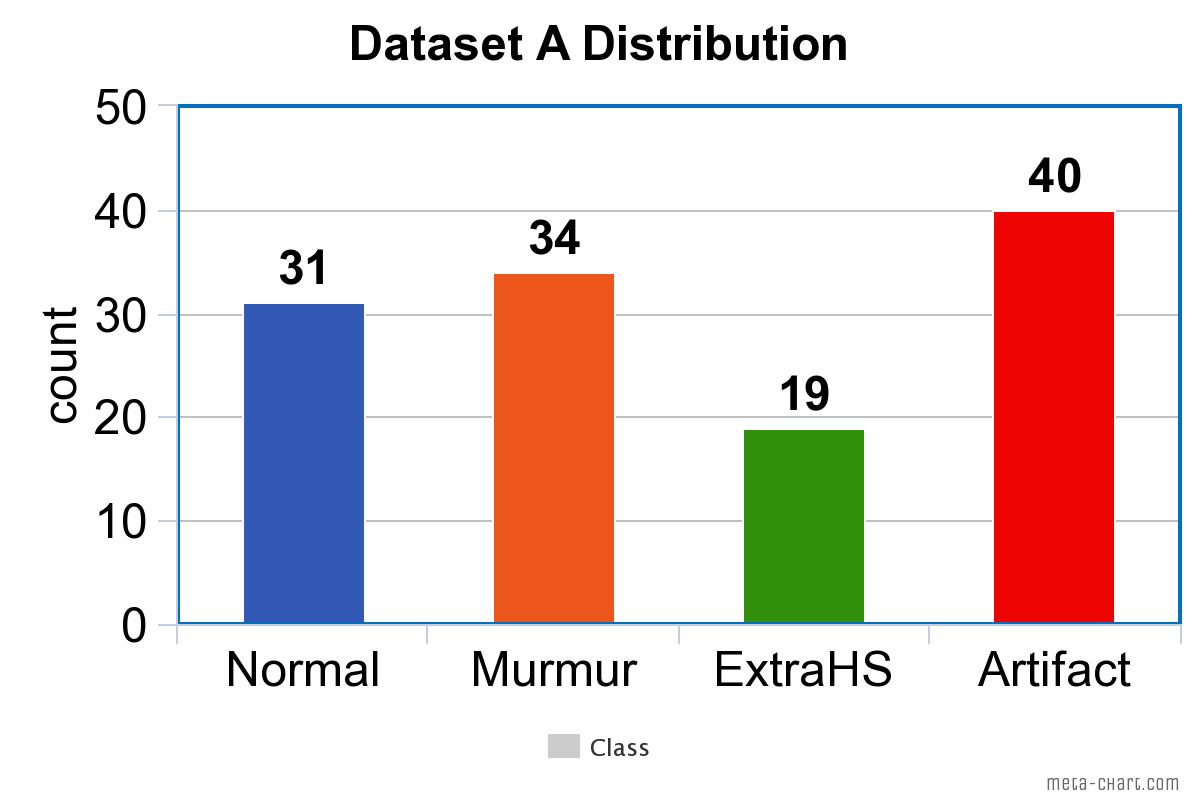
\includegraphics[scale = 0.13]{AAUgraphics/da.png}
			\end{figure}
			
			\column{0.5\textwidth}
			%   \only<1>{
			\begin{itemize}
				\item Recorded by the general public
				\item Device - iStethoscope Pro Iphone app
				\item Sampling Freq - 44100Hz
				\item Contains excessive background noise
			\end{itemize}{}
			%}
		\end{columns}
	\end{block}
}

\only<2>{
	
	\begin{block}{Dataset B}
		
		\begin{columns}
			\column{0.5\textwidth}
			\begin{figure}
				\centering
				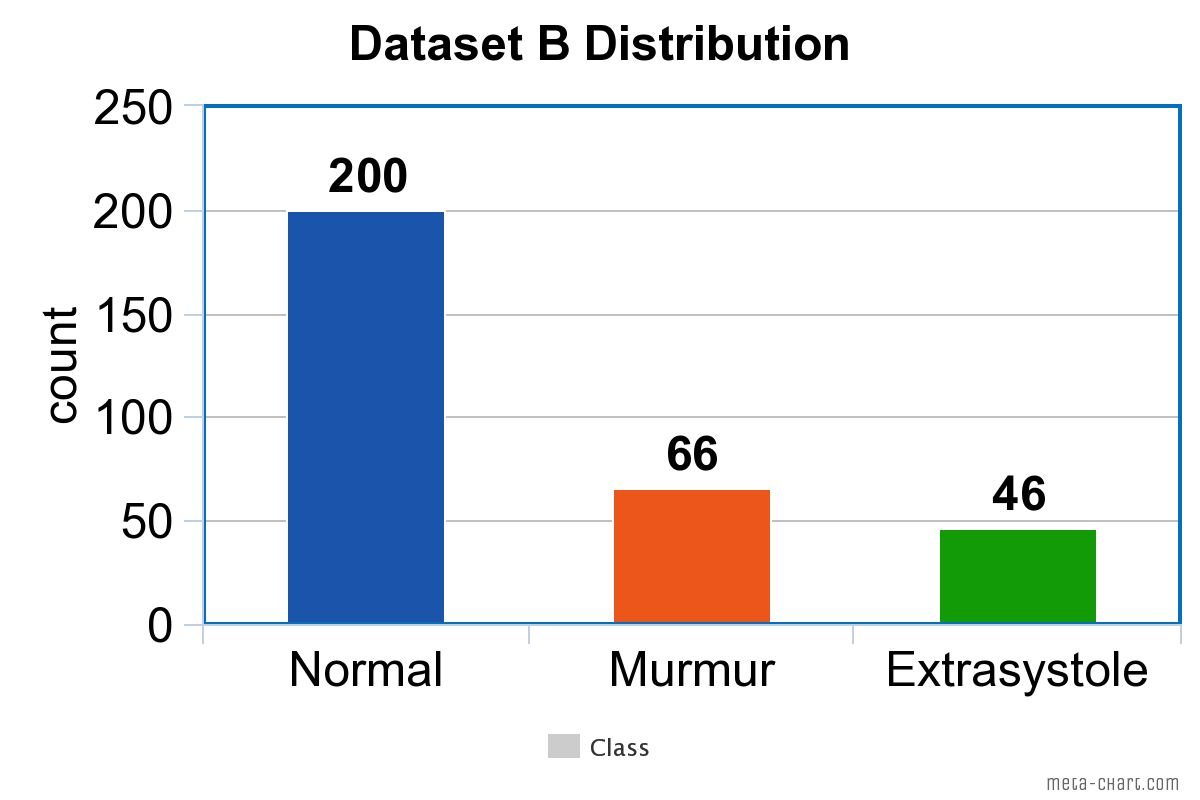
\includegraphics[scale = 0.13]{AAUgraphics/db.png}
			\end{figure}
			\column{0.5\textwidth}
			
			\begin{itemize}
				\item Recorded from a hospital by Medical Practitioners
				\item Device - Digital Stethoscope
				\item Sampling Freq - 4000Hz
				\item Contains background noise
			\end{itemize}
			
		\end{columns}
	\end{block}  
}
\end{frame}

%%%%%%%%%%%%%%%%%%%%%%%%%%%%%%%%%


\subsection{System Overview}
% general installation instructions
\begin{frame}{Methodology}{System Overview}
\begin{figure}
	\centering
	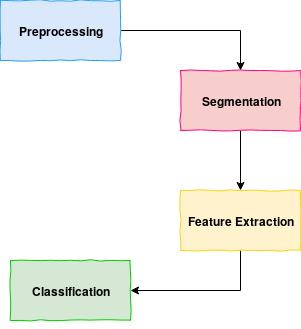
\includegraphics[scale = 0.5]{AAUgraphics/presentation.png}
\end{figure}{}
\end{frame}

%%%%%%%%%%%%%%%%%%%%%%%%%%%%%%%%%%%%%


\subsection{Preprocessing}
% general installation instructions
\begin{frame}{Methodology}{Preprocessing}
% \begin{block}
\begin{columns}
	\column{0.5\textwidth}
	\begin{enumerate}
		\item Downsample to 2kHz
		\item Bandpass Chebyshev filter [30Hz-195Hz]
		\item Normalization [-1 1]
		\item Wavelet Decomposition (db7 level 5)
		\item Refilter with LPF [195Hz]
	\end{enumerate}{}
	
	\column{0.5\textwidth}
	\only<1>{
		\begin{figure}
			\centering
			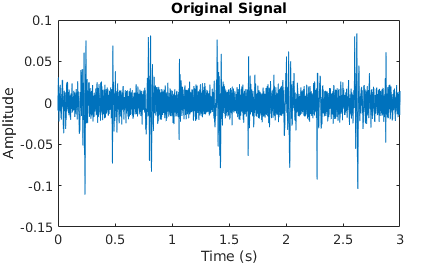
\includegraphics[width=0.87\textwidth]{AAUgraphics/originalp.png}
		\end{figure}
		
		\begin{figure}
			\centering
			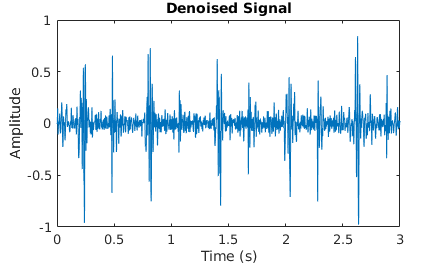
\includegraphics[width=0.87\textwidth]{AAUgraphics/denoisedp.png}
		\end{figure}
		
	}
\end{columns}


%\end{block}
\end{frame}



\end{document}
